%%%%%%%%%%%%%%%%%%%%%%%%%%%%%%%%%%%%%%%%%%%%%%%%%%%%%%%%%%%%%%%%%%%%%
%
% CSCI 1430 Written Question Template
%
% This is a LaTeX document. LaTeX is a markup language for producing documents. 
% You will fill out this document, compile it into a PDF document, then upload the PDF to Gradescope. 
%
% To compile into a PDF on department machines:
% > pdflatex thisfile.tex
%
% If you do not have LaTeX, your options are:
% - VSCode extension: https://marketplace.visualstudio.com/items?itemName=James-Yu.latex-workshop
% - Online Tool: https://www.overleaf.com/ - most LaTeX packages are pre-installed here (e.g., \usepackage{}).
% - Personal laptops (all common OS): http://www.latex-project.org/get/ 
%
% If you need help with LaTeX, please come to office hours.
% Or, there is plenty of help online:
% https://en.wikibooks.org/wiki/LaTeX
%
% Good luck!
% Srinath and the 1430 staff
%
%%%%%%%%%%%%%%%%%%%%%%%%%%%%%%%%%%%%%%%%%%%%%%%%%%%%%%%%%%%%%%%%%%%%%

\documentclass[11pt]{article}

\usepackage[english]{babel}
\usepackage[utf8]{inputenc}
\usepackage{amssymb}
\usepackage{xcolor}
\usepackage[colorlinks = true,
            linkcolor = blue,
            urlcolor  = blue]{hyperref}
\usepackage[a4paper,margin=1.5in]{geometry}
\usepackage{stackengine,graphicx}
\usepackage{fancyhdr}
\setlength{\headheight}{15pt}
\usepackage{microtype}
\usepackage{times}
\usepackage[shortlabels]{enumitem}
\setlist[enumerate]{topsep=0pt}
\usepackage{amsmath}
\usepackage{framed}
\usepackage{mdframed}
\usepackage{xcolor}
\usepackage[most]{tcolorbox}

% setup for todo lists:
\usepackage{enumitem}
\newlist{todolist}{itemize}{2}
\setlist[todolist]{label=$\square$}
\usepackage{pifont}
\newcommand{\cmark}{\ding{51}}%
\newcommand{\done}{\rlap{$\square$}{\raisebox{2pt}{\large\hspace{1pt}\cmark}}%
\hspace{-2.5pt}}

% a great python code format: https://github.com/olivierverdier/python-latex-highlighting
\usepackage{pythonhighlight}

\usepackage{trimclip,lipsum}

\frenchspacing
\setlength{\parindent}{0cm} % Default is 15pt.
\setlength{\parskip}{0.3cm plus1mm minus1mm}

\pagestyle{fancy}
\fancyhf{}
\lhead{Homework 0 Questions}
\rhead{CSCI 1430}
\lfoot{\textcolor{red}{\textbf{Only}
\ifcase\thepage
\or \textbf{instructions}
\or \textbf{A1}
\or \textbf{A2}
\or \textbf{A3}
\or \textbf{A4 (a) (i)}
\or \textbf{A4 (a) (ii) and A4 (b) (i)}
\or \textbf{A4 (b) (ii)}
\or \textbf{A5 (a) and A5 (b) (i)}
\or \textbf{A5 (b) (ii) and A5 (c)}
\or \textbf{Q6}
\or \textbf{A6}
\or \textbf{A7}
\or \textbf{A7}
\or \textbf{feedback}
\else
\textbf{[ERROR: PAGE MISALIGNMENT]}
\fi
\textbf{should be on this page}
}}
\rfoot{\thepage~/ 14}


\date{}

\title{\vspace{-1cm}Homework 0 Questions}


\begin{document}
\maketitle
\vspace{-3cm}
\thispagestyle{fancy}

\section*{ Document Instructions}
\begin{itemize}

  \item 7 questions \textbf{[4 + 4 + 8 + 6 + 4 + 3 + 3 = 32 points]}.
  \item Fill all your answers within the answer boxes, and \textbf{please do NOT remove the answer box outlines}.
  \item Questions are highlighted in the \textbf{orange boxes}, bonus questions are highlighted in \textbf{blue boxes}, answers should be recorded in the \textbf{green boxes}.
  \item Include code, images, and equations where appropriate.
  \item To identify all places where your responses are expected, search for `TODO'.
  \item The answer box sizes have been set by the staff beforehand and will truncate your text if it goes beyond the limit. Please make sure your responses fit in the appropriate spaces. \textbf{Extra pages are not permitted unless otherwise specified.}
  \item Make sure your submission has the right number of pages to validate page alignment sanity (check the footer).
  \item Please make this document anonymous.
\end{itemize}

\section*{ Gradescope Instructions}
\begin{itemize}
  \item When you are finished, compile this document to a PDF and submit it directly to Gradescope. 
  \item The pages will be automatically assigned to the right questions on Gradescope \textit{assuming you do not add any unnecessary pages}. \textbf{Inconsistently assigned pages will lead to a deduction of 2 points per misaligned page (capped at a maximum 6 point deduction).}
\end{itemize}

\pagebreak


\paragraph{Q1:} \textbf{[4 points]}
\begin{tcolorbox}[colback=orange!5!white,colframe=orange!75!black]
For each of the following, complete the task and check the box to mark it as done.
\end{tcolorbox}

\begin{tcolorbox}[colback=white!5!white,colframe=green!75!black]
%%%%%%% ANSWER STARTS HERE %%%%%%%%%%%%%%%%%%%%%%%%%%%%
TODO: Check off all items %%%%%% Remove this line in your answer! %%%%%%

\begin{todolist}
    \item[\done] This is an example of a checked box
    \item Read the GitHub tutorial \href{https://browncsci1430.github.io/webpage/resources/github_guide/}{here}.
    \item Create a GitHub account, if you don't have one.
    \item Join the \href{https://www.gradescope.com/}{Gradescope} course.
    \item Join the course \href{https://edstem.org/us/courses/28039/discussion/}{Ed}.
    \item Set up the \href{https://browncsci1430.github.io/webpage/resources/python_setup/}{python environment and virtual environment}.
    \item Set up an editing environment (e.g.,~\href{https://browncsci1430.github.io/webpage/resources/vscode_ssh/}{VSCode}), get it to use your python virtual environment, and know how to debug within it by setting breakpoints.
    \item Read the \href{https://browncsci1430.github.io/webpage/resources/python_tutorial/}{Python tutorial}.
%%%%%%% ANSWER ENDS HERE %%%%%%%%%%%%%%%%%%%%%%%%%%%%%%
\end{todolist}
\end{tcolorbox}

\pagebreak

\paragraph{Q2:} 
\textbf{[4 points]}
\begin{tcolorbox}[colback=orange!5!white,colframe=orange!75!black]
Please find and read the course collaboration policy on the \href{https://browncsci1430.github.io/webpage/policies/}{course website} and mark whether each of the following scenarios violates the policy.
\end{tcolorbox}

\emph{Note:} To fill in boxes, replace `\textbackslash square' with `\textbackslash blacksquare' for your answer.

\begin{enumerate}[(a)]
\item
Another cs1430 student looking at your code to help you debug, after you have spent time trying to tackle the bug or have come to TA office hours/Ed.

\begin{tcolorbox}[colback=white!5!white,colframe=green!75!black]
%%%%%%% ANSWER STARTS HERE %%%%%%%%%%%%%%%%%%%%%%%%%%%%
TODO: Check the right option %%%%%% Remove this line in your answer! %%%%%%

\begin{tabular}[h]{ll}
$\square$ & Acceptable \\
$\square$ & Violation \\
\end{tabular}
%%%%%%% ANSWER ENDS HERE %%%%%%%%%%%%%%%%%%%%%%%%%%%%%%
\end{tcolorbox}

\item
Using the result images from another student's code for your write up because your code is broken.

\begin{tcolorbox}[colback=white!5!white,colframe=green!75!black]
%%%%%%% ANSWER STARTS HERE %%%%%%%%%%%%%%%%%%%%%%%%%%%%
TODO: Check the right option %%%%%% Remove this line in your answer! %%%%%%

\begin{tabular}[h]{ll}
$\square$ & Acceptable \\
$\square$ & Violation \\
\end{tabular}
%%%%%%% ANSWER ENDS HERE %%%%%%%%%%%%%%%%%%%%%%%%%%%%%%
\end{tcolorbox}

\item
Googling third party sites to clarify concepts for written and code assignments, with proper citation.

\begin{tcolorbox}[colback=white!5!white,colframe=green!75!black]
%%%%%%% ANSWER STARTS HERE %%%%%%%%%%%%%%%%%%%%%%%%%%%%
TODO: Check the right option %%%%%% Remove this line in your answer! %%%%%%

\begin{tabular}[h]{ll}
$\square$ & Acceptable \\
$\square$ & Violation \\
\end{tabular}
%%%%%%% ANSWER ENDS HERE %%%%%%%%%%%%%%%%%%%%%%%%%%%%%%
\end{tcolorbox}

\item
A student who has previously taken the course and is not currently a TA sharing code with you to help you get through a bug.

\begin{tcolorbox}[colback=white!5!white,colframe=green!75!black]
%%%%%%% ANSWER STARTS HERE %%%%%%%%%%%%%%%%%%%%%%%%%%%%
TODO: Check the right option %%%%%% Remove this line in your answer! %%%%%%

\begin{tabular}[h]{ll}
$\square$ & Acceptable \\
$\square$ & Violation \\
\end{tabular}
%%%%%%% ANSWER ENDS HERE %%%%%%%%%%%%%%%%%%%%%%%%%%%%%%
\end{tcolorbox}

\end{enumerate}



%%%%%%%%%%%%%%%%%%%%%%%%%%%%%%%%%%%

% Please leave the pagebreak
\pagebreak

\paragraph{Q3:} \textbf{[8 points]} Computer vision is all around us, sometimes in surprising ways. Answer the following questions so we can get to know you better :)

\begin{enumerate}[(a)]
    \item 
\textbf{[2 points]} 
\begin{tcolorbox}[colback=orange!5!white,colframe=orange!75!black]
If you could have any computer vision related superpower, with no limitations, what would it be and how would you use it? \textbf{[2-3 sentences]}
\end{tcolorbox}

\begin{tcolorbox}[colback=white!5!white,colframe=green!75!black]
    \setbox0=\hbox{\parbox[t]{\textwidth}{
        %%%%%%% ANSWER STARTS HERE %%%%%%%%%%%%%%%%%%%%%%%%%%%%
        
        TODO: Your answer for (a) here %%%%%% Remove this line in your answer! %%%%%%
        
        %%%%%%% ANSWER ENDS HERE %%%%%%%%%%%%%%%%%%%%%%%%%%%%%%
        }}
        \clipbox{0pt \dimexpr\dp0-4\baselineskip\relax{} 0in 0pt}{\copy0}
\end{tcolorbox}



    \item \textbf{[6 points]}
All students enter the course with different backgrounds in socially responsible computing. Please first review our \href{https://browncsci1430.github.io/webpage/resources/ethics_guide/}{ethics primer} that introduces basic concepts to everyone.

    \begin{enumerate}[(i)]
    \item \textbf{[3 points]}
    \begin{tcolorbox}[colback=orange!5!white,colframe=orange!75!black]
    
    List at least one value that is at stake if you use your superpower as intended. Explain your reasoning. \textbf{[2-3 sentences]}
    \end{tcolorbox}
    
    \begin{tcolorbox}[colback=white!5!white,colframe=green!75!black]
        \setbox0=\hbox{\parbox[t]{\textwidth}{
            %%%%%%% ANSWER STARTS HERE %%%%%%%%%%%%%%%%%%%%%%%%%%%%
            
            TODO: Your answer for (b) here %%%%%% Remove this line in your answer! %%%%%%
            
            %%%%%%% ANSWER ENDS HERE %%%%%%%%%%%%%%%%%%%%%%%%%%%%%%
            }}
            \clipbox{0pt \dimexpr\dp0-5\baselineskip\relax{} 0in 0pt}{\copy0}
    \end{tcolorbox}
    \item \textbf{[3 points]}
    \begin{tcolorbox}[colback=orange!5!white,colframe=orange!75!black]
    
    List at least one value that is at stake if your archenemy misused your superpower. Explain your reasoning. \textbf{[2-3 sentences]}
    \end{tcolorbox}
    
    \begin{tcolorbox}[colback=white!5!white,colframe=green!75!black]
        \setbox0=\hbox{\parbox[t]{\textwidth}{
            %%%%%%% ANSWER STARTS HERE %%%%%%%%%%%%%%%%%%%%%%%%%%%%
            
            TODO: Your answer for (b) here %%%%%% Remove this line in your answer! %%%%%%
            
            %%%%%%% ANSWER ENDS HERE %%%%%%%%%%%%%%%%%%%%%%%%%%%%%%
            }}
            \clipbox{0pt \dimexpr\dp0-5\baselineskip\relax{} 0in 0pt}{\copy0}
    \end{tcolorbox}
    
    \end{enumerate}

\end{enumerate}



% Please leave the pagebreak
\pagebreak
\paragraph{Q4:} \textbf{[6 points]} Here is an image: \href{run:images/grizzlypeak-grayscale.png}{grizzlypeak-grayscale.png} (in the images folder)

\begin{enumerate}[(a)]
    \item 
    \begin{enumerate}[(i)] \item
\textbf{[2 points]}
Below is some code that sets pixels that have a value of 50 or less to 0. This removes some of the lower-intensity haze around the bright lights. However, the code only works on single-channel grayscale images.

\begin{tcolorbox}[colback=orange!5!white,colframe=orange!75!black]
Using a for loop and other appropriate modifications, convert the following code to work on \href{run:images/grizzlypeak-color.png}{grizzlypeak-color.png} (also in the images folder).
\end{tcolorbox}

\begin{tcolorbox}[enhanced jigsaw,pad at break*=1mm,colback=white!5!white,colframe=green!75!black,height=10cm]
\begin{python}
from skimage import io

A = io.imread('grizzlypeak-grayscale.png')
height, width = A.shape

# TODO: introduce a for loop that allows this 
# code to work on RGB images
for i in range(height):
    for j in range(width):
        if A[i,j] <= 50 :
            A[i,j] = 0
\end{python}
\end{tcolorbox}

\item
\textbf{[1 points]} Let's find the time it takes to run this operation once. Because a single short task on multitasking computers often takes variable time, we can record how long code execution takes on a small number of images and then average the execution time.

\begin{tcolorbox}[colback=orange!5!white,colframe=orange!75!black]
Record how long it takes to execute 10 times. How long does it take to change the pixel values once? Please include your code.
\end{tcolorbox}

\emph{Note: } When measuring the time, please ignore the file loading. You should only time the image modification itself.

\begin{tcolorbox}[colback=white!5!white,colframe=green!75!black,height=10cm]
\begin{python}
# TODO: your code here
\end{python}
    \setbox0=\hbox{\parbox[t]{\textwidth}{
    %%%%%%% ANSWER STARTS HERE %%%%%%%%%%%%%%%%%%%%%%%%%%%%
        
    TODO: Your answer for (a) (ii) here %%%%%% Remove this line in your answer! %%%%%%
    
    %%%%%%% ANSWER ENDS HERE %%%%%%%%%%%%%%%%%%%%%%%%%%%%%%
    }}
    \clipbox{0pt \dimexpr\dp0-1\baselineskip\relax{} 0in 0pt}{\copy0}
\end{tcolorbox}

\end{enumerate}

\item \textbf{[3 points]} Let's say we want to run our image modification 1000 times. If we used our current implementation, it would be really slow. Why might that be? We think we can find a faster solution.

\begin{enumerate}[(i)]
\item \textbf{[2 point]}
\begin{tcolorbox}[colback=orange!5!white,colframe=orange!75!black] 
Using logical indexing (see the Python tutorial), find a faster solution to remove the haze. 
\end{tcolorbox}

\begin{tcolorbox}[colback=white!5!white,colframe=green!75!black,height=3cm]
    \begin{python}
    # TODO: Your code here
    \end{python}
\end{tcolorbox}

\item \textbf{[1 point]}
\begin{tcolorbox}[colback=orange!5!white,colframe=orange!75!black]
Now, using your optimized solution, record how long it takes to change the pixel values 1000 times. How long does the new code take to change the pixel values on one image? How much faster is the new version per image, as a
multiplicative factor (eg: 2×, 5×)? Please include your code.
\end{tcolorbox}

\begin{tcolorbox}[colback=white!5!white,colframe=green!75!black,height=10cm]
\begin{python}
# TODO: your code here
\end{python}
    \setbox0=\hbox{\parbox[t]{\textwidth}{
    %%%%%%% ANSWER STARTS HERE %%%%%%%%%%%%%%%%%%%%%%%%%%%%
        
    TODO: Your answer for (b) (ii) here %%%%%% Remove this line in your answer! %%%%%%
    
    %%%%%%% ANSWER ENDS HERE %%%%%%%%%%%%%%%%%%%%%%%%%%%%%%
    }}
    \clipbox{0pt \dimexpr\dp0-1\baselineskip\relax{} 0in 0pt}{\copy0}
\end{tcolorbox}

\end{enumerate}
\end{enumerate}

%%%%%%%%%%%%%%%%%%%%%%%%%%%%%%%%%%%

% Please leave the pagebreak
\pagebreak
    \paragraph{Q5:} \textbf{[4 points]} Your friend tries to write code which reads in an image and displays it. 
    
    \begin{python}
        from skimage import io
        import matplotlib.pyplot as plt
        import numpy as np

        I = io.imread('gigi.jpg').astype(float32)
        plt.imshow(I)
        plt.show()
    \end{python}
    
    However, when they run the code, the image is almost entirely white. Confused, they come to you for help.

\begin{enumerate} [(a)]
    \item \textbf{[1 point]}
\begin{tcolorbox}[colback=orange!5!white,colframe=orange!75!black]
Why is the image being displayed incorrectly? \emph{Hint: check the data type of the image and the range of the numbers being read in}
\end{tcolorbox}

\begin{tcolorbox}[colback=white!5!white,colframe=green!75!black, height=3cm]
    %%%%%%% ANSWER STARTS HERE %%%%%%%%%%%%%%%%%%%%%%%%%%%%
        
    TODO: Your answer for (a) here %%%%%% Remove this line in your answer! %%%%%%

    %%%%%%% ANSWER ENDS HERE %%%%%%%%%%%%%%%%%%%%%%%%%%%%%%

\end{tcolorbox}

\item \textbf{[2 points]} You and your friend think of two possible ways to display the image correctly: making sure all of the floats are in the correct range (0 - 1) or using integers instead of floats.
\begin{enumerate} [(i)]

\item \textbf{[1 point]}
\begin{tcolorbox}[colback=orange!5!white,colframe=orange!75!black]
Write a possible fix that still uses the float data type.
\end{tcolorbox}

\begin{tcolorbox}[colback=white!5!white,colframe=green!75!black, height=4cm]
\begin{python}
# TODO: your code here
\end{python}
\end{tcolorbox}

\item \textbf{[2 point]}
\begin{tcolorbox}[colback=orange!5!white,colframe=orange!75!black]
Write a possible fix using the signed integer data type.
\end{tcolorbox}

\begin{tcolorbox}[colback=white!5!white,colframe=green!75!black, height=4cm]
\begin{python}
# TODO: your code here
\end{python}
\end{tcolorbox}
\end{enumerate}

\item \textbf{[1 point]} Another friend comes to you and wants help darkening an image. With your newly functioning image display code, you decide to help!
\begin{tcolorbox}[colback=orange!5!white,colframe=orange!75!black]
Using your answer from part (b) (ii), read in 'gigi.png', darken the pixel intensities by 50, and display the new image. Include your code and a screenshot of the darkened image.
\end{tcolorbox}

\begin{tcolorbox}[colback=white!5!white,colframe=green!75!black,height fill]
    \begin{python}
    # TODO: your code here
    \end{python}
    
    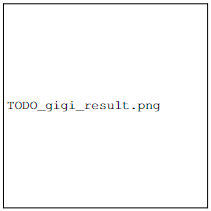
\includegraphics[width=0.5\textwidth,height=7cm,keepaspectratio]{images/TODO_gigi_result.png}

\end{tcolorbox}
\end{enumerate}


%%%%%%%%%%%%%%%%%%%%%%%%%%%%%%%%%%%

% Please leave the pagebreak
\pagebreak
\paragraph{Q6:} \textbf{[2 + 1 points]}

The debugger within VSCode is an important tool you can use to discover potential bugs in the code that you right.

Imagine our task is to create a crop of an image that starts at the center of the image and extends to the lower right corner of the image. If all goes well, we should only see content from the lower right region of the original image.

\emph{Image:} \href{images/gigi.jpg}{gigi.jpg} (in images folder)

\begin{python}
from skimage import io
import matplotlib.pyplot as plt

origImage = io.imread('gigi.jpg')
(height, width, channels) = origImage.shape
startCropX = width % 2
startCropY = height % 2
croppedImage = origImage[startCropY:, startCropX:]

plt.imshow(croppedImage)
plt.show()
\end{python}

\begin{tcolorbox}[colback=orange!5!white,colframe=orange!75!black,enhanced jigsaw,breakable,pad at break*=1mm]
Create a new python file in the same directory as the image, and copy in the above code block. Then, open the file in VSCode, and execute the code within a debugging session by pressing F5 (or `Run $\rightarrow$ Start Debugging'). At the prompt, we wish to `Debug the currently active Python file'.

The output is not currently what we want, so let's stop execution and then identify the bug in this program:
\begin{enumerate}
    \item First, set a breakpoint at line 7 and then re-execute the code within a debugging session.
    \item Inspect the `startCropX' variable either by looking at the left-hand Variables panel, or by mouse hovering over the variable in the text editor. What should it be?
    \item Execute line 7 of code by `stepping over' the current line (F10, or `Run $\rightarrow$ Step Over). We should now be about to execute line 8.
    \item Inspect `startCropY' and verify its correctness.
\end{enumerate}

At this point, you might have an idea of how to fix the code. But, before stopping execution and editing the file, let's test out our hypothesis in the `Debug Console' during debugging.

\begin{enumerate}
    \item Switch to the Debug Console by pressing CTRL-SHIFT-Y (or `View $\rightarrow$ Debug Console') --- you should see it in the bottom right of the display screen.
    \item \emph{This is an interactive Python console with access to working memory.} As a test, print out the value of `width'. Perform a mathematical operation on `width'.
    \item Assign the right value to `startCropX' within the Debug Console. Notice how the value updated in the Variables panel.
    \item Do the same for `startCropY'.
    \item From this point, execute the rest of the code by Continuing beyond our current paused position in the code. Press F5 to Continue (or `Run $\rightarrow$ Continue').
\end{enumerate}

Re-execute the debugger, and capture a screenshot showing your use of the Debug Console and inspection of a variable. Also, write the correct code below.
\end{tcolorbox}

\begin{tcolorbox}[colback=white!5!white,colframe=green!75!black,height=8cm,height fill]
    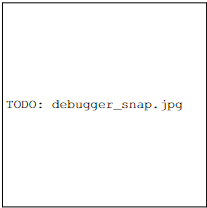
\includegraphics[width=0.5\textwidth,height=7cm,keepaspectratio]{images/TODO_debugger_snap.jpg}
    
    \begin{python}
    # TODO: paste your code here 
    \end{python}
\end{tcolorbox}



%%%%%%%%%%%%%%%%%%%%%%%%%%%%%%%%%%%
\pagebreak
\paragraph{Q7:} \textbf{[2 + 1 points]} This program should print out the maximum value in the matrix obtained by multiplying a random non-square matrix with its transpose.

Here, we're using some numpy functions that may be new to us, but they each have self-explanatory names.

\begin{python}
import numpy as np
from numpy import random as r

mat_1 = r.rand(200,150)
mat_2 = mat_1
np.transpose(mat_2)
mat_3 = np.matmul(mat_1, mat_2)
mat_max = np.max(mat_3)

print("Max value:", mat_max)
\end{python}

This time, when we execute the code, it will raise an exception.

\begin{tcolorbox}[colback=orange!5!white,colframe=orange!75!black]
Run the code in a debugging session, note the exception, and inspect the variables. Form a hypothesis for the error, and use the Debug Console to test that it prevents the exception. 
\end{tcolorbox}

\emph{Hint: Remember rules about matrix multiplication. What should the dimensions of each matrix be? Use the debugger to notice how the shapes of the images do or do not change.}

Capture a screenshot of your session showing us the issue and paste the correct code.

\begin{tcolorbox}[colback=white!5!white,colframe=green!75!black,breakable,height=15cm,enhanced jigsaw,pad at break*=1mm]
    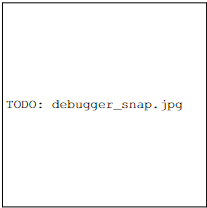
\includegraphics[width=0.5\textwidth,height=7cm,keepaspectratio]{images/TODO_debugger_snap.jpg}
    
    \begin{python}
    # TODO: paste your code here
    
    
    
    
    
    
    
    
    
    
    
    
    
    
    
    ################################################
    # YOU MAY USE THIS ADDITIONAL SPACE
    
    # WARNING: IF YOU DON'T END UP USING THIS SPACE
    # KEEP THESE COMMENTS TO MAINTAIN PAGE ALIGNMENT
    ################################################
    \end{python}
    
\end{tcolorbox}

% %%%%%%%%%%%%%%%%%%%%%%%%%%%%%%%%%%%
%% any suggestions for more?
\pagebreak
\section*{Feedback? (Optional)}
Please help us make the course better. If you have any feedback for this assignment, we'd love to hear it!
\end{document}
